\documentclass[11pt]{article}

% ---------- Packages ----------
\usepackage[utf8]{inputenc}
\usepackage[T1]{fontenc}
\usepackage{lmodern}
\usepackage[margin=1in]{geometry}
\usepackage{graphicx}
\usepackage{xcolor}
\usepackage{listings}
\usepackage{hyperref}
\usepackage{enumitem}
\usepackage{titlesec}
\usepackage{parskip}

% ---------- Hyperref setup ----------
\hypersetup{
    colorlinks=true,
    linkcolor=blue!60!black,
    urlcolor=blue!60!black,
    citecolor=blue!60!black,
    pdftitle={Quick GF180 MCU Inverter Tutorial in the IIC-OSIC Container},
    pdfauthor={James Stine}
}

% ---------- Listings setup for shell code ----------
\definecolor{shellbg}{RGB}{245,245,245}
\definecolor{shellrule}{RGB}{200,200,200}
\definecolor{shellcomment}{RGB}{0,128,0}
\definecolor{shellkeyword}{RGB}{0,0,180}

\lstdefinestyle{shell}{
    backgroundcolor=\color{shellbg},
    basicstyle=\ttfamily\small,
    breaklines=true,
    breakatwhitespace=false,
    columns=fullflexible,
    frame=single,
    rulecolor=\color{shellrule},
    showstringspaces=false,
    keepspaces=true,
    xleftmargin=0pt,
    framexleftmargin=4pt,
    framexrightmargin=4pt,
    framextopmargin=4pt,
    framexbottommargin=4pt,
    aboveskip=8pt,
    belowskip=8pt,
    language=bash,
    commentstyle=\color{shellcomment},
    keywordstyle=\color{shellkeyword}\bfseries,
}
\lstset{style=shell}

\usepackage{xcolor}
\usepackage{tcolorbox}

\newtcbox{\inlinecode}{on line,
  colback=gray!12,
  colframe=gray!12,
  boxrule=0pt,
  arc=2pt,
  left=2pt,
  right=2pt,
  top=1pt,
  bottom=1pt,
  boxsep=1pt
}
\usepackage{caption}
\usepackage{url}
\usepackage{hyperref}
\usepackage{subcaption}
\usepackage[hypcap=false]{caption}
\usepackage{float}

% ---------- Section formatting ----------
\titleformat{\section}{\Large\bfseries}{\thesection}{1em}{}
\titleformat{\subsection}{\large\bfseries}{\thesubsection}{1em}{}

% ---------- Title ----------
\title{Step-by-Step Tutorial for an Automated GF180MCU Digital Design Workflow}
\author{Maryam Shahangian and James E. Stine \\
        Oklahoma State University\\
        Electrical and Computer Engineering Department\\
        Stillwater, OK 74078 USA\\
        \texttt{\{maryam.shahangian, james.stine\}@okstate.edu}}
\date{}

\begin{document}
\maketitle

% ============================================================
\section{Introduction}

The goal of this tutorial is to provide a simple, step-by-step workflow for running OpenROAD inside a containerized environment. The tutorial first introduces the basic concept of a container and explains why containerized environments are useful for digital design workflows. A container provides a ready-to-use environment in which the required design tools are already installed and configured. As a result, users do not need to manually install tools or resolve software dependency issues.

The tutorial then demonstrates how OpenROAD can automate the major stages of a digital design flow. Rather than executing each stage manually, OpenROAD-flow-scripts can guide the design from RTL input through synthesis, place-and-route, and final GDSII layout generation.

To demonstrate the workflow, the tutorial first uses an example design that is already included within OpenROAD. This provides a complete example of the design flow inside the container, beginning with the RTL design files and ending with the generated GDSII layout. Finally, the tutorial explains how the same flow can be adapted to use the
\href{https://github.com/stineje/globalfoundries-pdk-libs-gf180mcu_osu_sc}{
\textcolor{blue!70!black}{\textbf{OSU GF180}}
}
standard-cell library.

% ============================================================
\section{Understanding the Environment}

In this tutorial, the design environment is provided through a containerized setup. This means that the chip-design tools are not installed directly on the host operating system. Instead, they are provided inside a prepared environment that can be launched consistently across different machines.
In practical terms, the host computer remains the user's normal system, while the actual design workflow runs inside a preconfigured software environment containing the required tools, libraries, scripts, and dependencies.

\subsection{What IIC-OSIC-TOOLS Is}

\href{https://github.com/iic-jku/iic-osic-tools}{
\textcolor{blue!70!black}{\textbf{IIC-OSIC-TOOLS}}
} is the containerized tool environment used in this tutorial. It provides an integrated, ready-to-use platform for IC design, with the required tools already bundled together. This makes setup easier and avoids the need to install and configure each tool manually.

\subsection{What Docker Does}

Docker is the software used to launch and manage the prepared environment. In simple terms, the container is the workspace that already contains the design tools, while Docker is the software that creates, starts, and manages that workspace. In this tutorial, Docker is used to run the IIC-OSIC-TOOLS container so that the OpenROAD workflow can be executed in a consistent and reproducible environment.
% ============================================================
\section{Installing Docker}

Docker Desktop installers are available for multiple operating systems and architectures. The official Docker download page provides installers for Windows, Linux, and macOS.
In this tutorial, the documented setup was performed on Windows. Therefore, the following steps focus specifically on the Windows installation path and the continuation of the environment setup.

\begin{enumerate}
    \item Download Docker Desktop from the official Docker website for the appropriate operating system.

\begin{figure}[H]
    \centering
    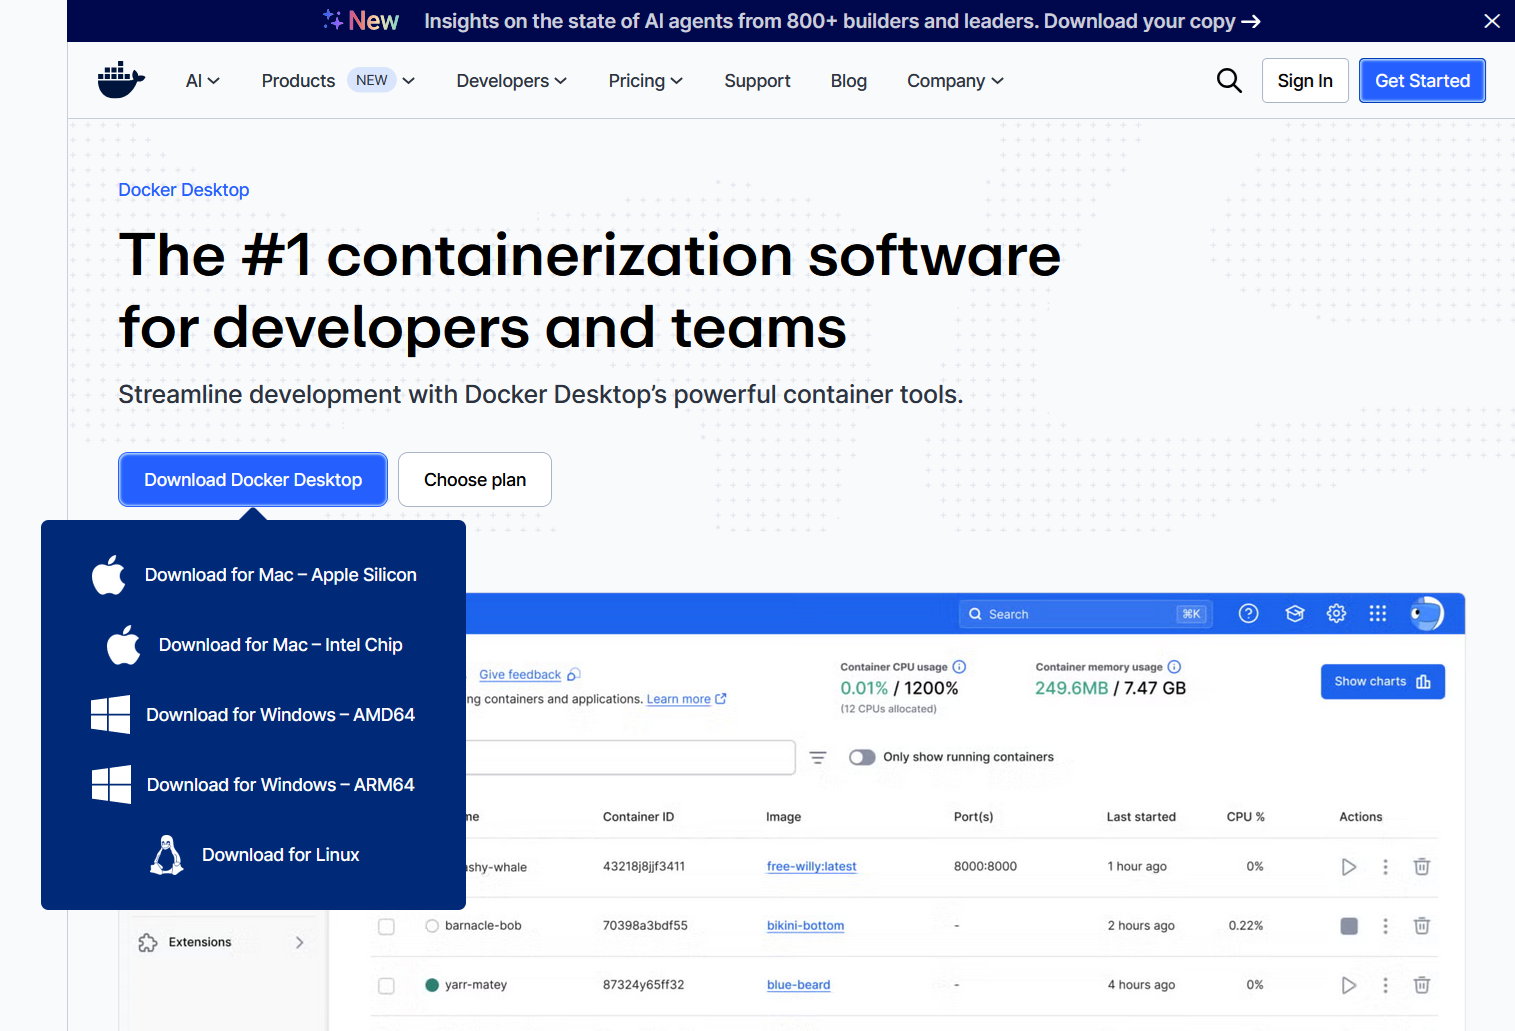
\includegraphics[width=0.80\textwidth]{1.png}
    \caption{Docker Desktop download page for selecting the appropriate installer.}
    \label{fig:docker-download}
\end{figure}
    
    \item Follow the installation instructions provided by Docker Desktop to complete the installation on the host machine.
\end{enumerate}

After Docker Desktop is installed, select the preferred method for accessing the container environment. Three access modes are available:

\begin{itemize}
    \item \textbf{VNC Mode:} Provides a full graphical desktop environment that can be accessed through a web browser.

    \item \textbf{Jupyter Mode:} Provides a web-based notebook environment useful for running commands, documenting steps, and working interactively.

    \item \textbf{Shell Mode:} Provides a simple command-line terminal for running scripts and server-side tasks.
\end{itemize}

For this tutorial, Jupyter Mode is selected as the primary access method.

\subsection{Select the Correct Chipathon Branch and Docker Image}

After cloning the repository, 
\begin{enumerate}
    \item open Command Prompt (CMD) and run the following commands:

\begin{lstlisting}
cd %USERPROFILE%\eda\designs\iic-osic-tools
\end{lstlisting}

\begin{lstlisting}
git checkout ieee_chipathon
\end{lstlisting}

This switches the repository to the branch used for the Chipathon setup.

\textbf{Note:} \inlinecode{DESIGNS=\$HOME/eda/designs}
(\inlinecode{DESIGNS=\%USERPROFILE\%\textbackslash eda\textbackslash designs} for \inlinecode{.bat})
sets the directory that holds your design files.
This directory is mounted into the container on \inlinecode{/foss/designs}.

\item Next, set the Docker image tag and start Jupyter:

\begin{lstlisting}
SET DOCKER_TAG=chipathon26
start_jupyter.bat
\end{lstlisting}

These commands switch to the Chipathon branch and start the Jupyter container using the Chipathon 26 image.

\item If a Jupyter container was already created previously using an older image, remove it first and then start it again:

\begin{lstlisting}
docker rm -f iic-osic-tools_jupyter
SET DOCKER_TAG=chipathon26
start_jupyter.bat
\end{lstlisting}

\begin{figure}[H]
    \centering
    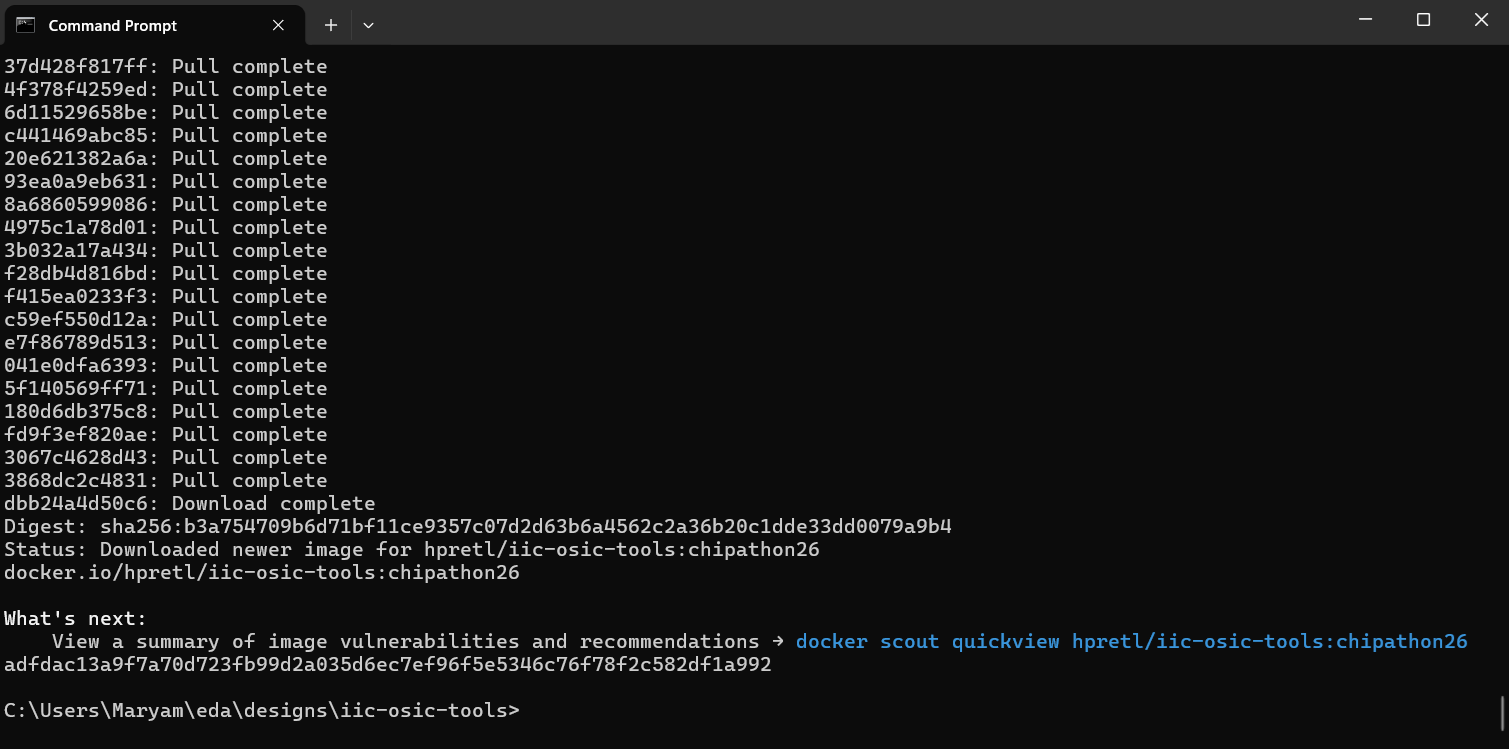
\includegraphics[width=0.55\textwidth]{7.png}
    \caption{Successful startup of the Chipathon 26 Jupyter container in Command Prompt.}
    \label{fig:jupyter-container-start}
\end{figure}


\item After that, open Docker Desktop. Click the Play button next to \texttt{iic-osic-tools\_jupyter} and wait a few seconds for the container to start.
Once the container is running, go to the \textbf{Ports} column and click \texttt{8888:8888} to open the Jupyter environment in a web browser.
\end{enumerate}

\begin{figure}[H]
    \centering
    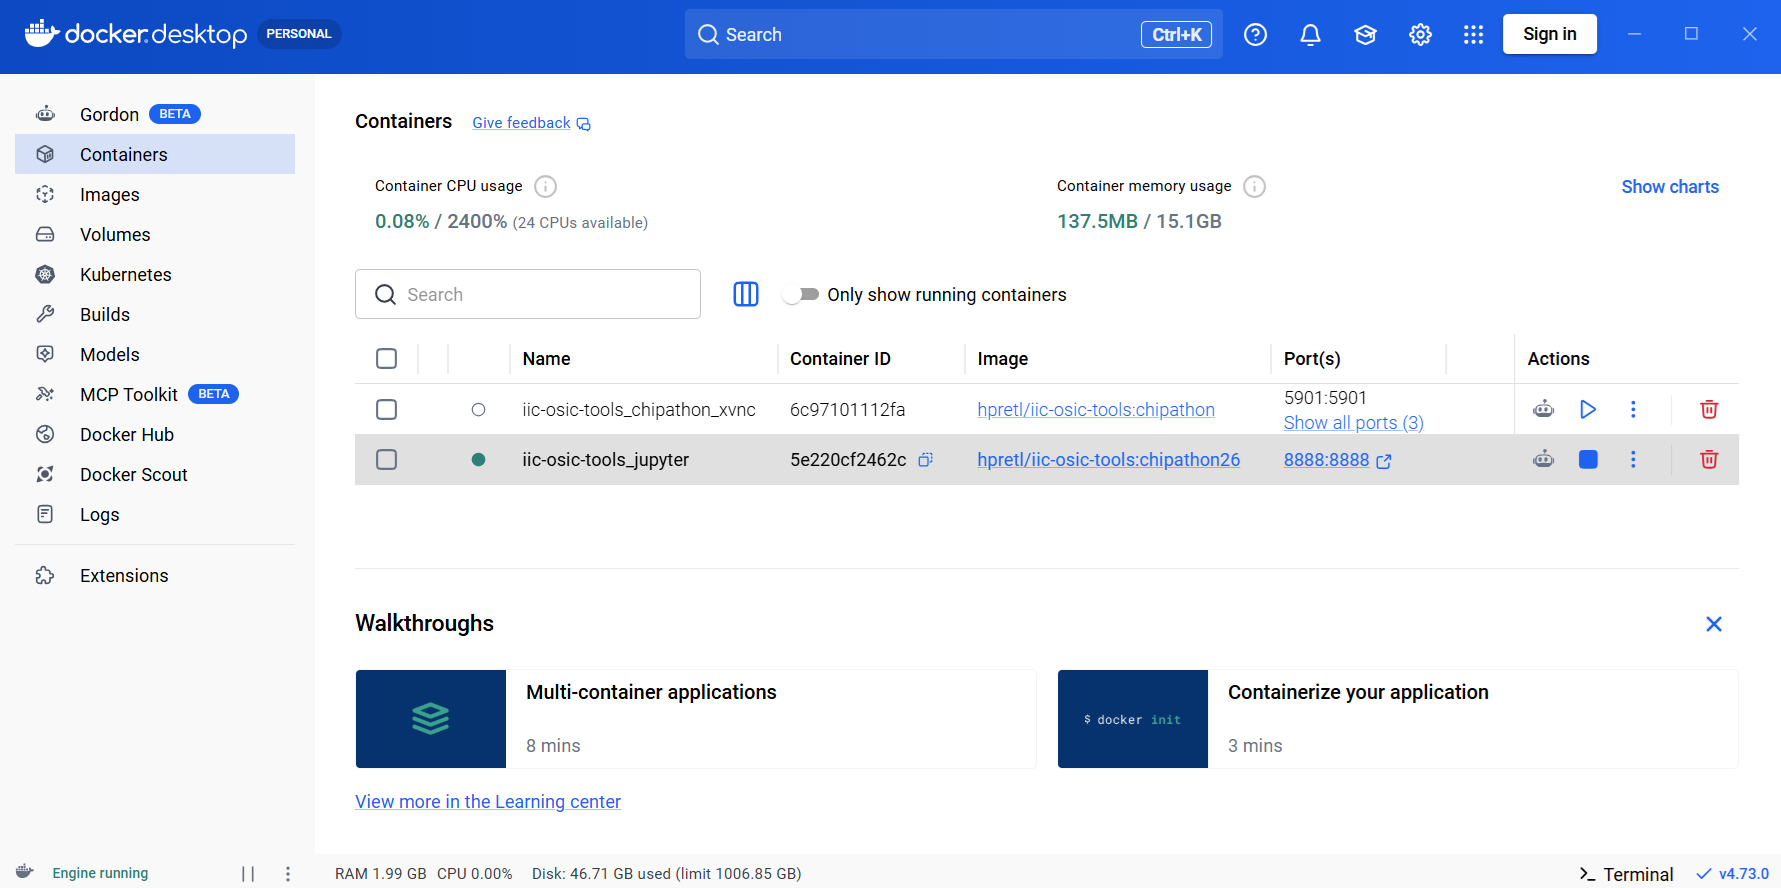
\includegraphics[width=0.55\textwidth]{2.png}
    \caption{Docker Desktop showing the running Jupyter container and the available port link.}
    \label{fig:docker-jupyter-port}
  \vspace{0.2cm}
    \centering
    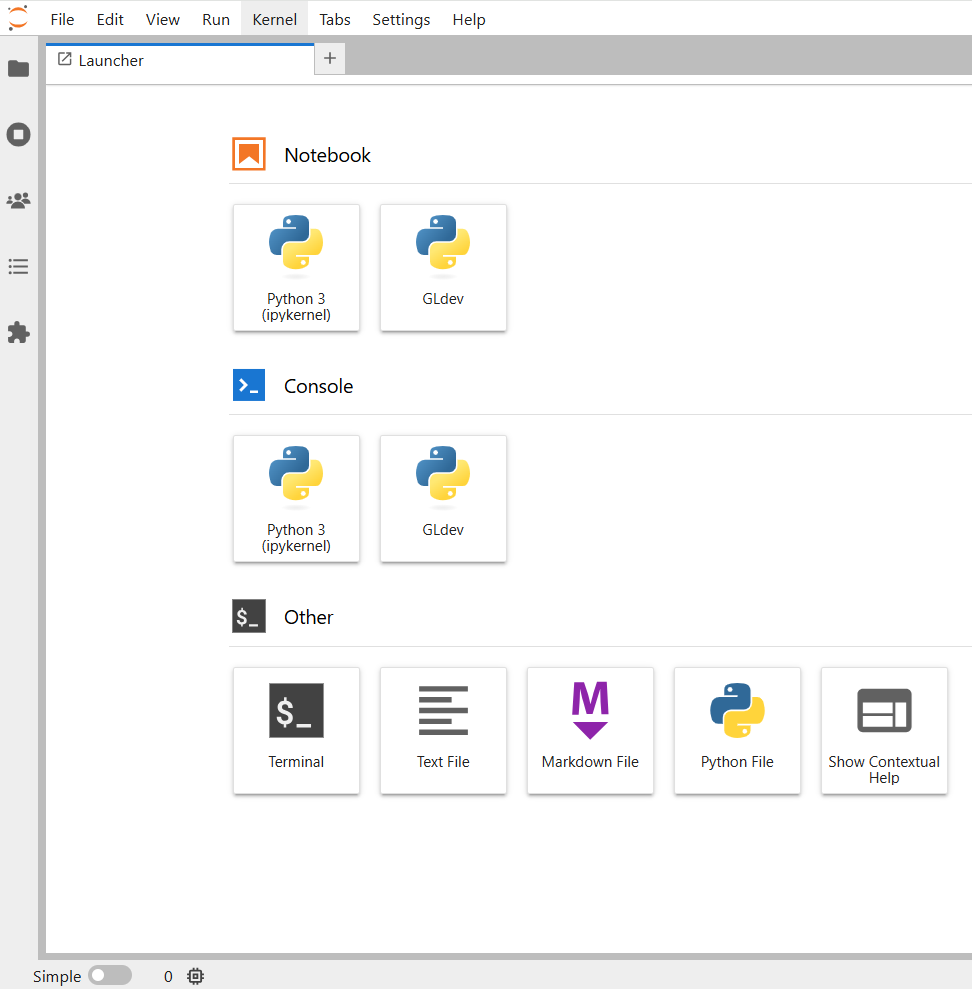
\includegraphics[width=0.50\textwidth]{3.png}
    \caption{JupyterLab launcher page after the container starts successfully.}
    \label{fig:jupyterlab-launcher}
\end{figure}

\textbf{Tip:} If the port number shown in Docker Desktop is not clickable, manually open a web browser and go to: \texttt{http://localhost:8888}

For VNC mode, click the corresponding VNC port link in Docker Desktop, or manually open: \texttt{http://localhost:80}
When prompted, enter the default password: \texttt{abc123}
At this point, the JupyterLab interface should become visible in the browser, indicating that the container environment has started successfully and is ready for interactive use.
The primary shared working directories are:

\begin{itemize}
    \item Windows:
    \texttt{C:\textbackslash Users\textbackslash <username>\textbackslash eda\textbackslash designs}

    \item Container:
    \texttt{/foss/designs}
\end{itemize}

Use this folder for all files and designs throughout the tutorial.
% ============================================================
\subsection{Check the Installed Tools}

To open a terminal in JupyterLab, go to the \textbf{Launcher} page and, under \textbf{Other}, click \textbf{Terminal}.
Then run the following commands:

\begin{lstlisting}
cd /foss/designs && pwd && ls
\end{lstlisting}

To verify the installed tools and display the ORFS commit version, run:

\begin{lstlisting}
yosys -V
\end{lstlisting}

\begin{lstlisting}
openroad -version
\end{lstlisting}

\begin{lstlisting}
echo $TOOLS
\end{lstlisting}

\begin{lstlisting}
cat $TOOLS/openroad/ORFS_COMMIT
\end{lstlisting}

These commands confirm that the required tools are available inside the container and display the matching ORFS commit used by the environment.

\textbf{What Is an “Image”?}

In Docker terminology, an image is a prebuilt software environment that already contains the required tools and dependencies.
In this tutorial, the \textbf{Chipathon26} image is used. This image is distributed through the IIC-OSIC-TOOLS environment and maintained by Harald Pretl and collaborators. It already includes the main tools required for the workflow, such as OpenROAD and Yosys.

\textbf{Why is the commit important?}

The ORFS commit helps confirm that the OpenROAD-flow-scripts version matches the OpenROAD tools installed inside the container. This avoids compatibility problems caused by version mismatches.

\subsection{Clone OpenROAD-flow-scripts}

Next, clone the \href{https://github.com/The-OpenROAD-Project/OpenROAD-flow-scripts.git}{
\textcolor{blue!70!black}{\textbf{OpenROAD-flow-scripts}}
} repository and check out the commit version stored in the container image.

\begin{lstlisting}
cd /foss/designs
\end{lstlisting}

\begin{lstlisting}
git clone https://github.com/The-OpenROAD-Project/OpenROAD-flow-scripts.git
\end{lstlisting}

\begin{lstlisting}
cd OpenROAD-flow-scripts
\end{lstlisting}

\begin{lstlisting}
git checkout $(cat $TOOLS/openroad/ORFS_COMMIT)
\end{lstlisting}

This ensures that the flow scripts match the OpenROAD tools provided by the container image.


\subsubsection{Setting the Tool Paths}
Now configure the tool paths so that the flow uses the OpenROAD and Yosys executables installed inside the container.

\begin{lstlisting}
cat >> ~/.bashrc <<'EOF'
export YOSYS_EXE=/foss/tools/yosys/bin/yosys
export OPENROAD_EXE=/foss/tools/openroad/bin/openroad
export OPENSTA_EXE=/foss/tools/openroad/bin/sta
EOF
\end{lstlisting}

\begin{lstlisting}
source ~/.bashrc
\end{lstlisting}

This configuration step only needs to be performed once. Afterward, the terminal session will automatically recognize these tool paths.


\textbf{Note:}
In this setup, the flow scripts expect the executables to exist under the local \texttt{tools/install} directory. However, the Chipathon 26 container already provides these tools under \texttt{/foss/tools}.

The following one-time setup creates symbolic links to the installed tools so that the OpenROAD flow can start normally.

\begin{lstlisting}
cd /foss/designs/OpenROAD-flow-scripts
mkdir -p tools/install
ln -sfn /foss/tools/yosys tools/install/yosys
ln -sfn /foss/tools/openroad tools/install/OpenROAD
\end{lstlisting}



\subsubsection{Run the Flow}

Move to the flow directory and run:

\begin{lstlisting}
cd /foss/designs/OpenROAD-flow-scripts/flow
\end{lstlisting}

\begin{lstlisting}
make
\end{lstlisting}

This starts the OpenROAD flow using the tool versions provided by the current Chipathon 26 container image.
At this stage, the OpenROAD environment inside the IIC-OSIC-TOOLS container is fully configured and ready for use.
The environment is now prepared so that the focus can shift to the main objective: running and understanding chip-design examples.

% ============================================================
\section{Run the AES Example Design}

In this section, the OpenROAD flow is tested using a ready-to-use example design provided by OpenROAD. This helps verify that the environment is functioning correctly before moving to custom designs.
The AES example is used here. The goal is not to modify the design, but to understand how the automated flow operates from RTL input to final layout generation.
The RTL source files for the example are located inside the \textbf{designs/src} directory. The platform-specific configuration files for AES are stored under the corresponding GF180 design directory.
First, move to the designs directory and enter the source folder:

\begin{lstlisting}
cd /foss/designs/OpenROAD-flow-scripts/flow/designs
cd src
ls
\end{lstlisting}

\begin{figure}[H]
    \centering
    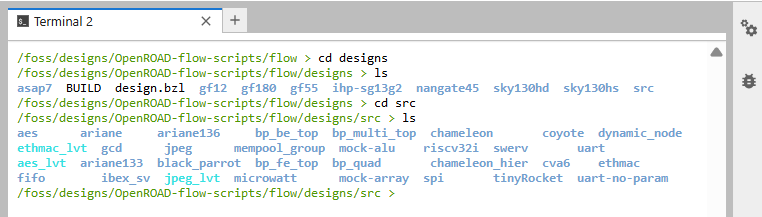
\includegraphics[width=1.00\textwidth]{10.png}
    \caption{Listing available example designs in OpenROAD-flow-scripts, including the AES design example.}
    \label{fig:aes-directory-files}
\end{figure}

In this directory, the available example designs can be seen. One of them is \textbf{aes}.
Next, move to the AES platform directory and list its files:

\begin{lstlisting}
cd /foss/designs/OpenROAD-flow-scripts/flow/designs/gf180/aes
ls
\end{lstlisting}

The main configuration files for the AES example can now be seen, including:

\begin{itemize}
    \item \texttt{config.mk}
    \item \texttt{constraint.sdc}
\end{itemize}

The \textbf{config.mk} file defines the primary design setup, while the \textbf{constraint.sdc} file contains the timing constraints used by the flow.
Before running the AES example, it is useful to briefly inspect the \textbf{config.mk} file.
This file contains the main configuration for the design, including the design name, target platform, Verilog source files, and timing constraints used during the flow.

\begin{figure}[H]
    \centering
    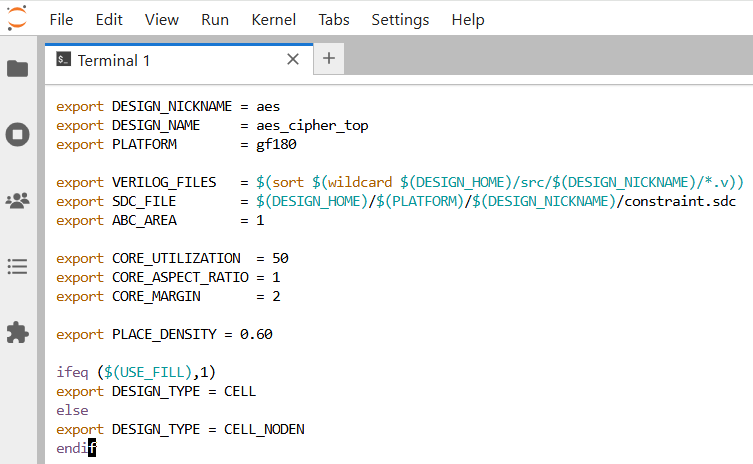
\includegraphics[width=0.75\textwidth]{11.png}
    \caption{Example contents of the AES \texttt{config.mk} file used to define the design, platform, RTL sources, and implementation settings.}
    \label{fig:aes-config-file}
\end{figure}

After that, move to the flow directory and run the AES example:

\begin{lstlisting}
cd /foss/designs/OpenROAD-flow-scripts/flow
\end{lstlisting}

\begin{lstlisting}
make DESIGN_CONFIG=./designs/gf180/aes/config.mk
\end{lstlisting}

As soon as this command is executed, the automated OpenROAD design flow begins.
The first major stage is \textbf{synthesis}, where the RTL description is converted into a gate-level netlist. This step is performed by \textbf{Yosys}.
After synthesis, the flow automatically continues through the remaining physical-design stages, including:

\begin{itemize}
    \item Floorplanning
    \item Placement
    \item Clock Tree Synthesis (CTS)
    \item Routing
\end{itemize}

These stages are executed sequentially without requiring manual intervention.
Depending on the complexity of the design and the available system resources, the complete flow may take several minutes to finish.


\begin{figure}[H]
    \centering
    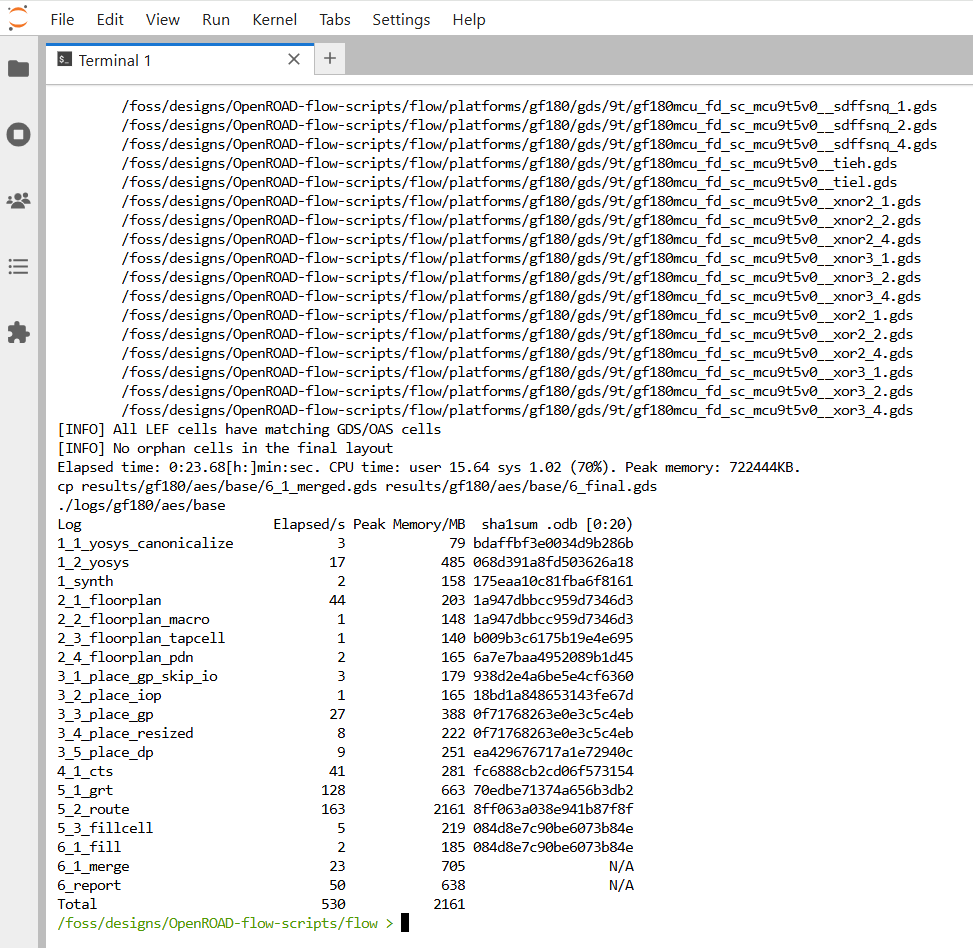
\includegraphics[width=0.9\textwidth]{12.png}
    \caption{Successful completion of the automated OpenROAD AES implementation flow, including synthesis, placement, CTS, routing, and final GDS generation.}
    \label{fig:aes-flow-complete}
\end{figure}

In Jupyter mode, the graphical interface may not appear because Jupyter provides a terminal-oriented environment rather than a full desktop interface.
To view the final layout graphically, either use the VNC mode or open the generated GDS file locally using KLayout.
A simple way to access the final layout is to download the generated GDS file directly from the JupyterLab file browser.
The generated GDS file is typically located at:

\begin{lstlisting}
/foss/designs/OpenROAD-flow-scripts/flow/results/gf180/aes/base/6_1_merged.gds
\end{lstlisting}

After downloading the file to the local computer, open it using \textbf{KLayout}.

\begin{figure}[H]
    \centering
    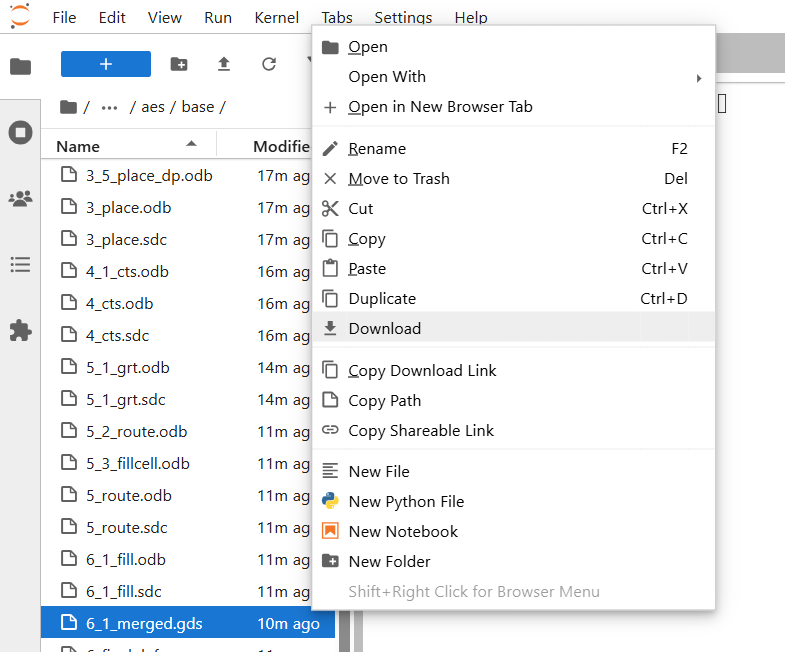
\includegraphics[width=0.60\textwidth]{13.png}
    \caption{Downloading the generated merged GDS file from JupyterLab and opening it locally with KLayout.}
    \label{fig:download-gds-klayout}
\end{figure}

\begin{figure}[H]
    \centering
    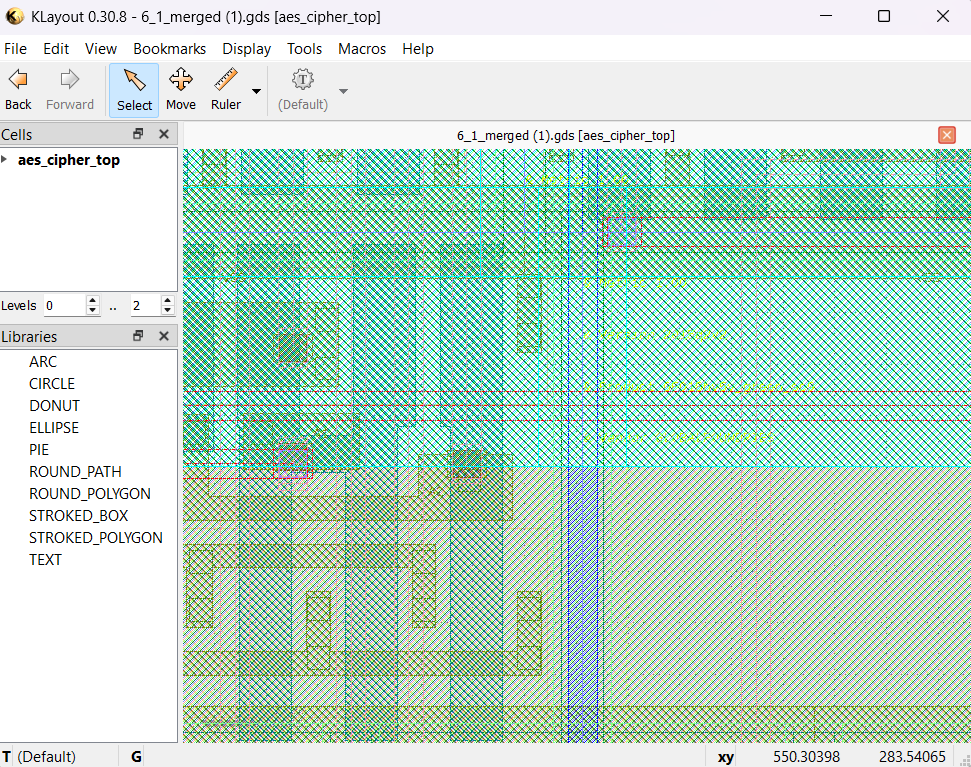
\includegraphics[width=0.60\textwidth]{15.png}
    \caption{Viewing the final AES GDS layout in KLayout after completing the automated OpenROAD flow.}
    \label{fig:aes-final-layout}
\end{figure}
% ============================================================
% ============================================================
\clearpage
\section{Worked Example: AES Implementation with the GF180MCU OSU Standard-Cell Library}

In the previous section, the built-in AES example provided by OpenROAD-flow-scripts was used to demonstrate the default automated implementation flow inside the container environment. That example served as a baseline for understanding how the flow operates using the standard design setup already available in OpenROAD.

In this section, the same AES design is reused, but the library environment is modified so that the design is implemented with the GF180MCU OSU standard-cell library instead of the default library configuration. The purpose of this worked example is to show how an existing OpenROAD example can be adapted to a different standard-cell library and then evaluated within the same containerized flow.

This approach is useful because it allows the effect of library substitution to be studied on a realistic design rather than on a minimal test case. Since AES is already available in the OpenROAD example set, it provides a convenient and meaningful benchmark for documenting the required configuration changes, the integration procedure, and the practical issues that arise during implementation.

The standard cells used in this work are taken from the GF180MCU OSU standard-cell library developed at Oklahoma State University. This library was designed by James E. Stine, Jr. and the VLSI Computer Architecture Research Group.

\subsection{Matching the OpenROAD Configuration to the OSU Library}

The AES RTL files and the related configuration files have to  organize so that they can be referenced consistently by the modified design setup. This step is important because the OpenROAD flow depends on a fixed directory structure and correctly referenced input files in order to recognize and process the design properly.

To use the GF180MCU OSU standard-cell library instead of the default library, the relevant OpenROAD configuration files must be updated in the proper locations. In this setup, the design-specific configuration is modified in the AES design directory, while the platform-level settings are adjusted in the GF180 platform directory.

The main design-level changes are made in the following file:
\begin{itemize}
    \item \texttt{/foss/designs/OpenROAD-flow-scripts/flow/designs/gf180/aes/config.mk}
\end{itemize}

\begin{figure}[H]
    \centering
    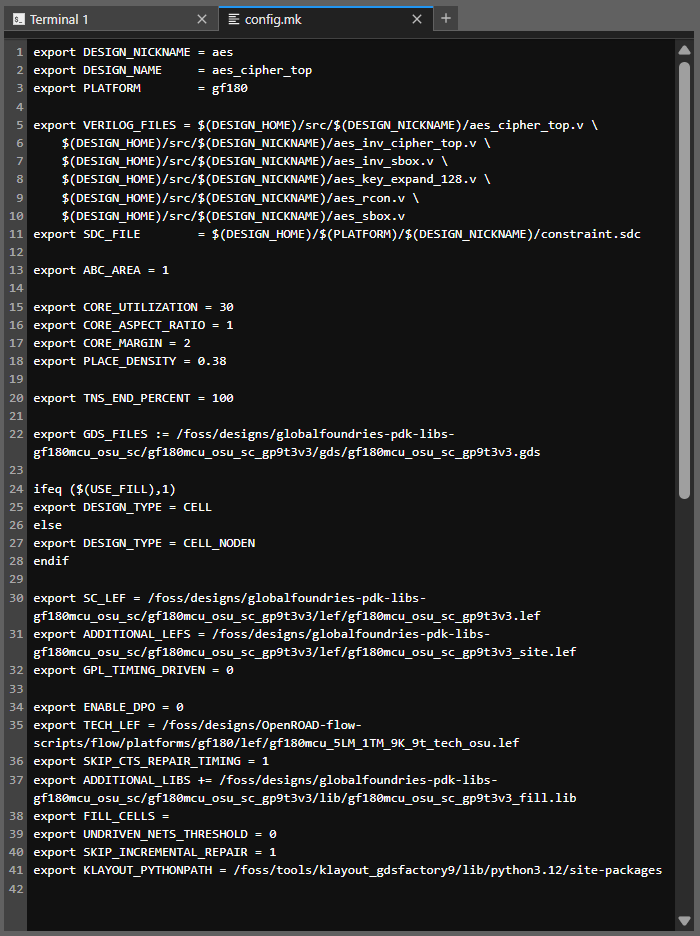
\includegraphics[width=0.75\textwidth, trim=0 120 0 0, clip]{config-aes.png}
    \caption{Modified AES \texttt{config.mk} file located under \texttt{flow/designs/gf180/aes}.}
    \label{fig:aes_osu_config}
\end{figure}

This file is updated so that the AES design points to the modified synthesized netlist, the OSU GDS file, the OSU standard-cell LEF, the OSU site LEF, and the technology LEF used for this library setup. In this way, the design is evaluated using the intended OSU library views rather than the default GF180 library configuration.

The platform-level changes are applied in:
\begin{itemize}
    \item \texttt{/foss/designs/OpenROAD-flow-scripts/flow/platforms/gf180/config.mk}
\end{itemize}

\begin{center}
    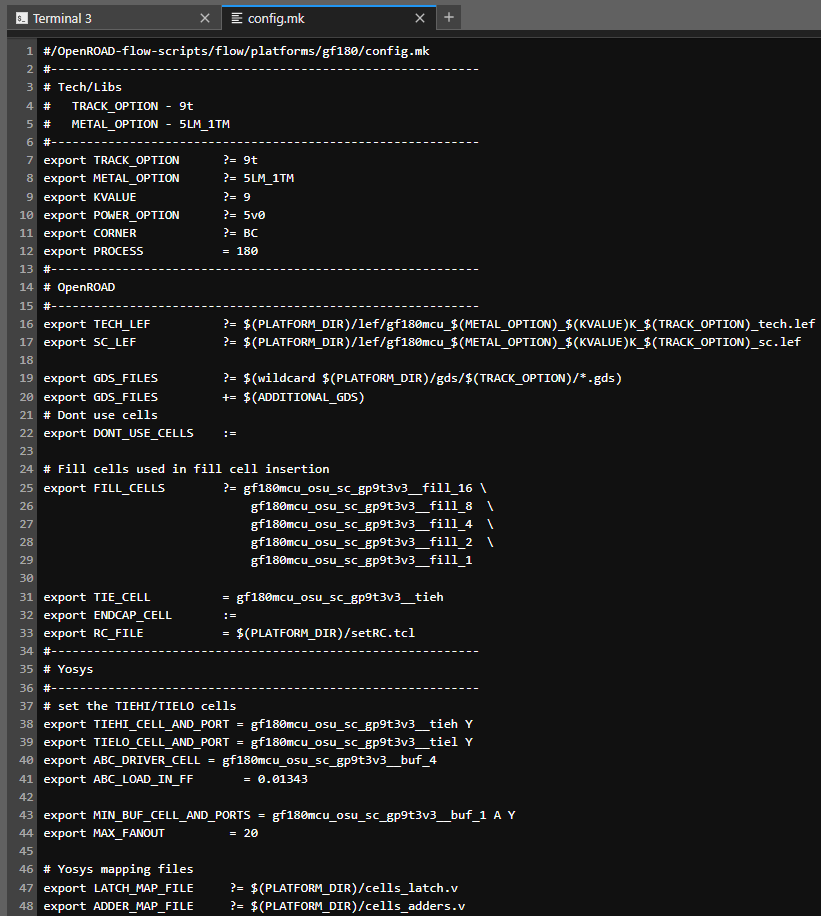
\includegraphics[width=0.60\textwidth]{osu3-1.png}

    \vspace{0.15cm}

    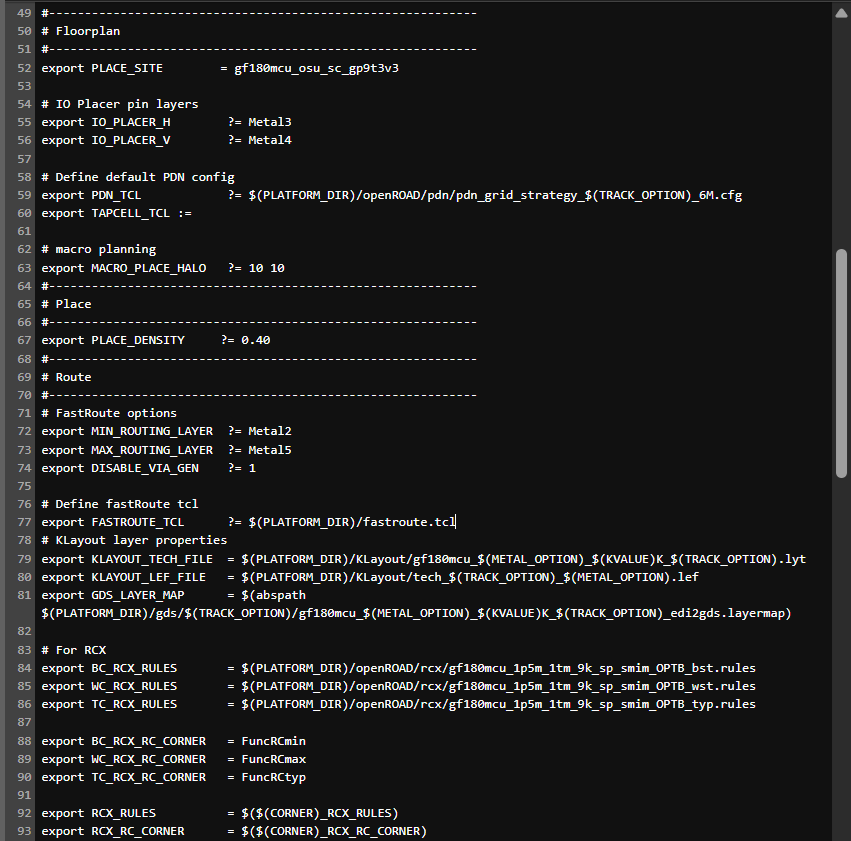
\includegraphics[width=0.60\textwidth]{osu3-2.png}

    \vspace{0.15cm}

    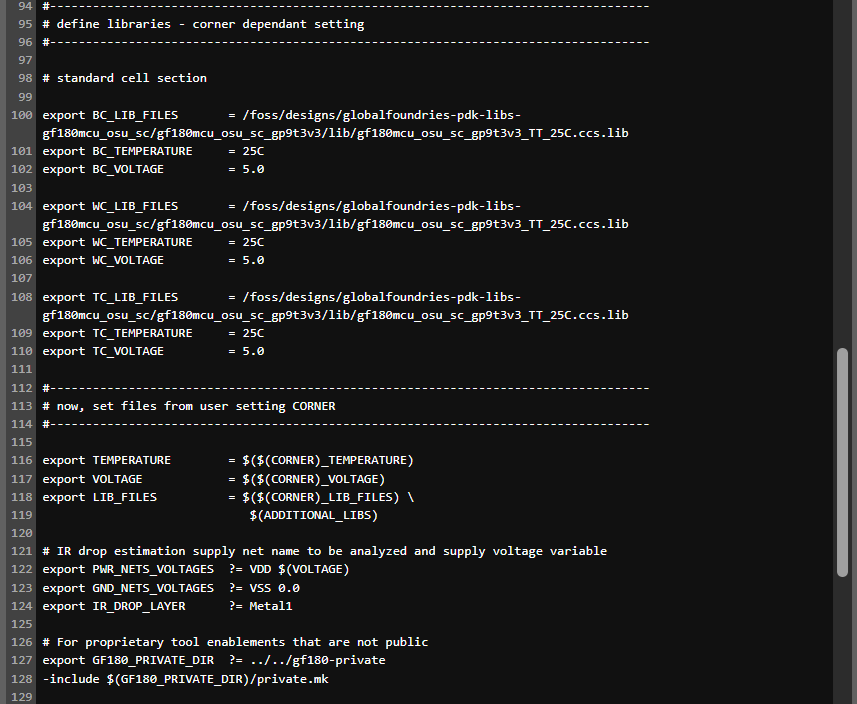
\includegraphics[width=0.70\textwidth]{osu3-3.png}

    \captionof{figure}{GF180 platform \texttt{config.mk} sections used for the GF180MCU OSU library integration.}
    \label{fig:gf180_platform_config}
\end{center}

This file defines the platform defaults used by the OpenROAD flow, including library-dependent settings such as filler cells, tie cells, and technology-level references. These settings must be checked carefully to ensure that they remain consistent with the selected OSU library.

In addition to the configuration files, the technology-mapping files must also be matched to the target library. In this example, the files
\texttt{cells\_adders.v} and \texttt{cells\_latch.v}, located under
\texttt{/foss/designs/OpenROAD-flow-scripts/flow/platforms/gf180/},
are reviewed and aligned with the GF180MCU OSU library.

This means that the mapped cells, instance names, and pin connections used in these files must correspond exactly to the cell names and pin names provided by the OSU library.

\begin{figure}[H]
    \centering

    \begin{subfigure}{0.55\textwidth}
        \centering
        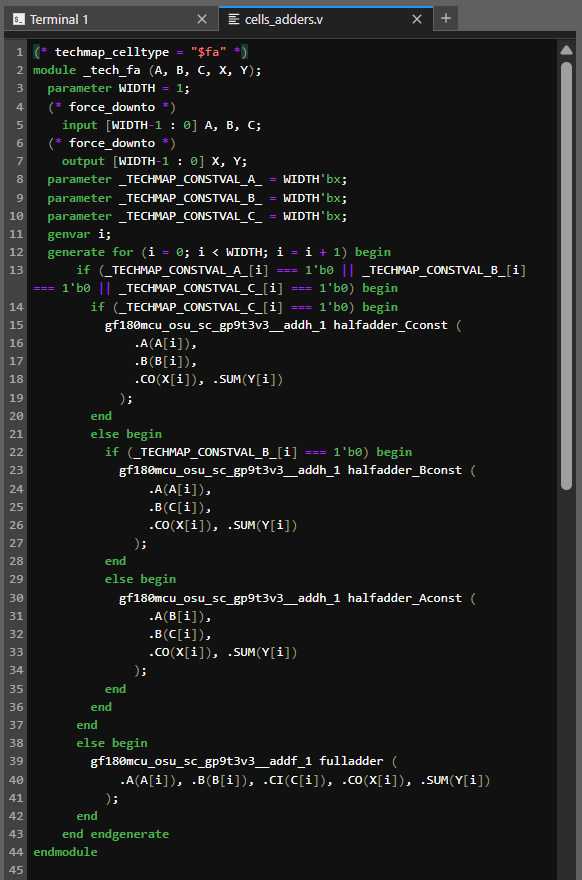
\includegraphics[width=\textwidth]{adder.png}
        \caption{\texttt{cells\_adders.v}}
        \label{fig:osu_adders}
    \end{subfigure}

    \vspace{0.3cm}

    \begin{subfigure}{0.53\textwidth}
        \centering
        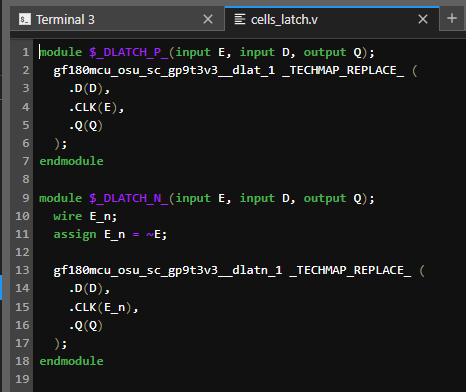
\includegraphics[width=\textwidth]{osu2.png}
        \caption{\texttt{cells\_latch.v}}
        \label{fig:osu_latch}
    \end{subfigure}

    \caption{Technology-mapping files aligned with the GF180MCU OSU standard-cell library.}
    \label{fig:osu_techmap_files}
\end{figure}

Therefore, integrating the AES example with the GF180MCU OSU standard-cell library requires both configuration-level changes and cell-mapping consistency checks. The design files, platform files, and mapping files must all refer to the same library views in order for the OpenROAD flow to process the design correctly.

After the configuration is completed, go to the flow directory and run:

\begin{lstlisting}
cd /foss/designs/OpenROAD-flow-scripts/flow
make DESIGN_CONFIG=./designs/gf180/aes/config.mk
\end{lstlisting}

If an error occurs during the flow, first fix the problem. Then remove the generated intermediate files and run the flow again from the same directory.

\begin{lstlisting}
cd /foss/designs/OpenROAD-flow-scripts/flow
make clean_all DESIGN_CONFIG=./designs/gf180/aes/config.mk
make DESIGN_CONFIG=./designs/gf180/aes/config.mk
\end{lstlisting}

If the flow completes successfully, the final result files should be visible in the AES output directory. In particular, files such as \texttt{6\_final.gds}, \texttt{6\_final.def}, \texttt{6\_final.v}, and \texttt{6\_final.sdc} should appear. This confirms that the main OpenROAD implementation stages have completed correctly with the GF180MCU OSU standard-cell library.
An example of the expected final output is shown in Figure~\ref{fig:osu_aes_final_results}.
If the flow completes successfully, the final result files should be visible in the AES output directory. In particular, files such as \texttt{6\_final.gds}, \texttt{6\_final.def}, \texttt{6\_final.v}, and \texttt{6\_final.sdc} should appear. This confirms that the main OpenROAD implementation stages have completed correctly with the GF180MCU OSU standard-cell library.

An example of the expected final output is shown in Figure~\ref{fig:osu_aes_final_results}.

\begin{figure}[H]
    \centering
    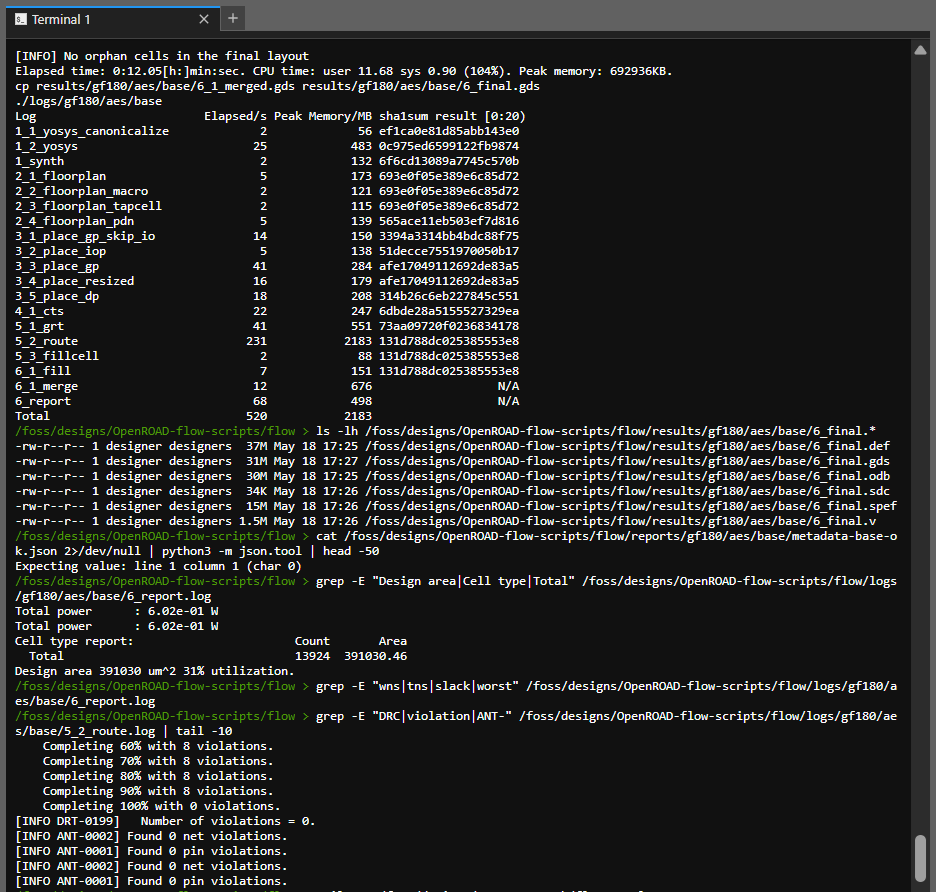
\includegraphics[width=0.90\textwidth]{result.png}
    \caption{Example of a successful AES run using the GF180MCU OSU standard-cell library, showing the generated final output files in the OpenROAD results directory.}
    \label{fig:osu_aes_final_results}
\end{figure}

In Jupyter mode, interactive layout inspection is less convenient because Jupyter primarily provides a terminal-based environment rather than a full graphical desktop interface. For this reason, if the goal is to inspect layout layers visually, there are two practical options. The first option is to download the generated GDS file from Jupyter and open it locally in KLayout. The second option is to use the VNC interface and view the layout directly inside the container.

If the VNC method is preferred, open a Windows Command Prompt and run:

\begin{lstlisting}
cd %USERPROFILE%\eda\designs\iic-osic-tools
SET DOCKER_TAG=chipathon26
start_vnc.bat
\end{lstlisting}

After the VNC container starts, open Docker Desktop and select the corresponding VNC port, as shown in Figure~\ref{fig:vnc_docker_port}. Then open the VNC session in a web browser. When the login prompt appears, enter the default password:

\begin{lstlisting}
abc123
\end{lstlisting}

\begin{figure}[H]
    \centering
    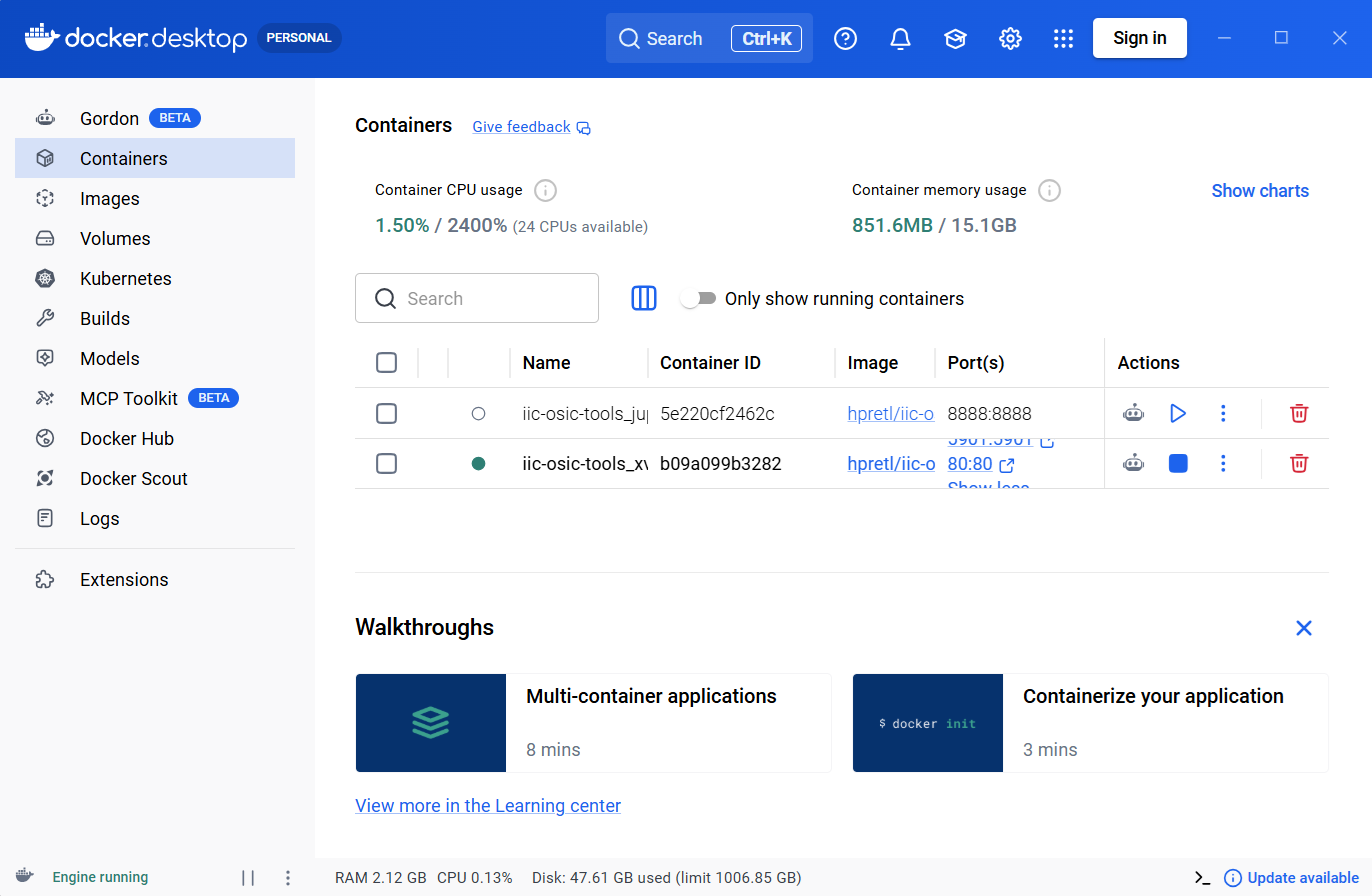
\includegraphics[width=0.85\textwidth]{vnc.png}
    \caption{Docker Desktop showing the running VNC container and the port used to open the graphical desktop session.}
    \label{fig:vnc_docker_port}
\end{figure}

Once the graphical desktop opens, right-click on the desktop background and open a terminal window inside the VNC session.

\begin{figure}[H]
    \centering
    
\includegraphics[width=0.65\textwidth]{open_terminal.png}
    \caption{Opening a terminal in the VNC session.}
    \label{fig:vnc_open_terminal}
\end{figure}

Then launch KLayout with:

\begin{lstlisting}
klayout /foss/designs/OpenROAD-flow-scripts/flow/results/gf180/aes/base/6_1_merged.gds
\end{lstlisting}

A full-chip view of the complete final GDS layout is shown in Figure~\ref{fig:osu_aes_complete_gds}.

\begin{figure}[H]
    \centering
    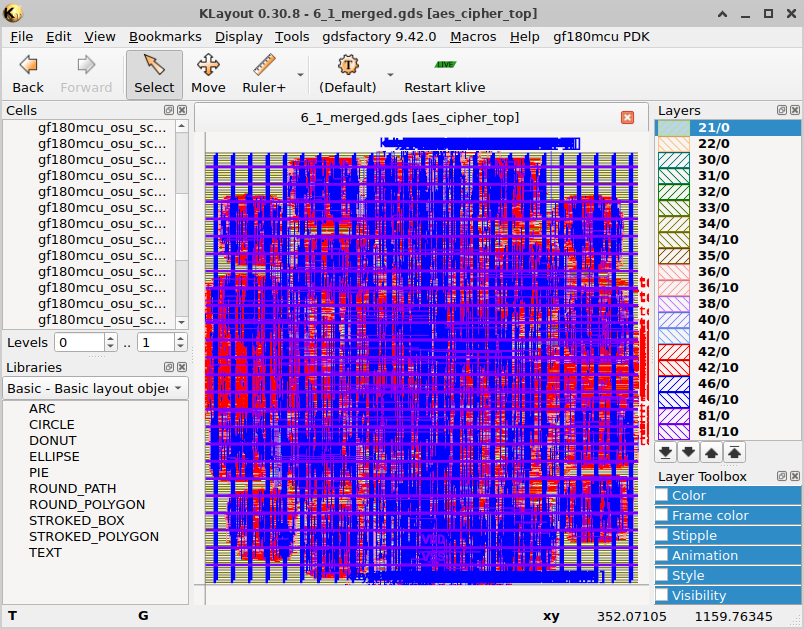
\includegraphics[width=0.75\textwidth]{complete_gds.png}
    \caption{Top-level view of the complete final AES GDS layout generated with the GF180MCU OSU standard-cell library, shown in KLayout.}
    \label{fig:osu_aes_complete_gds}
\end{figure}

The zoomed-in view in Figure~\ref{fig:klayout_osu_layout} shows the layout in greater detail and makes the OSU standard cells visible inside the final design.

\begin{figure}[H]
    \centering
    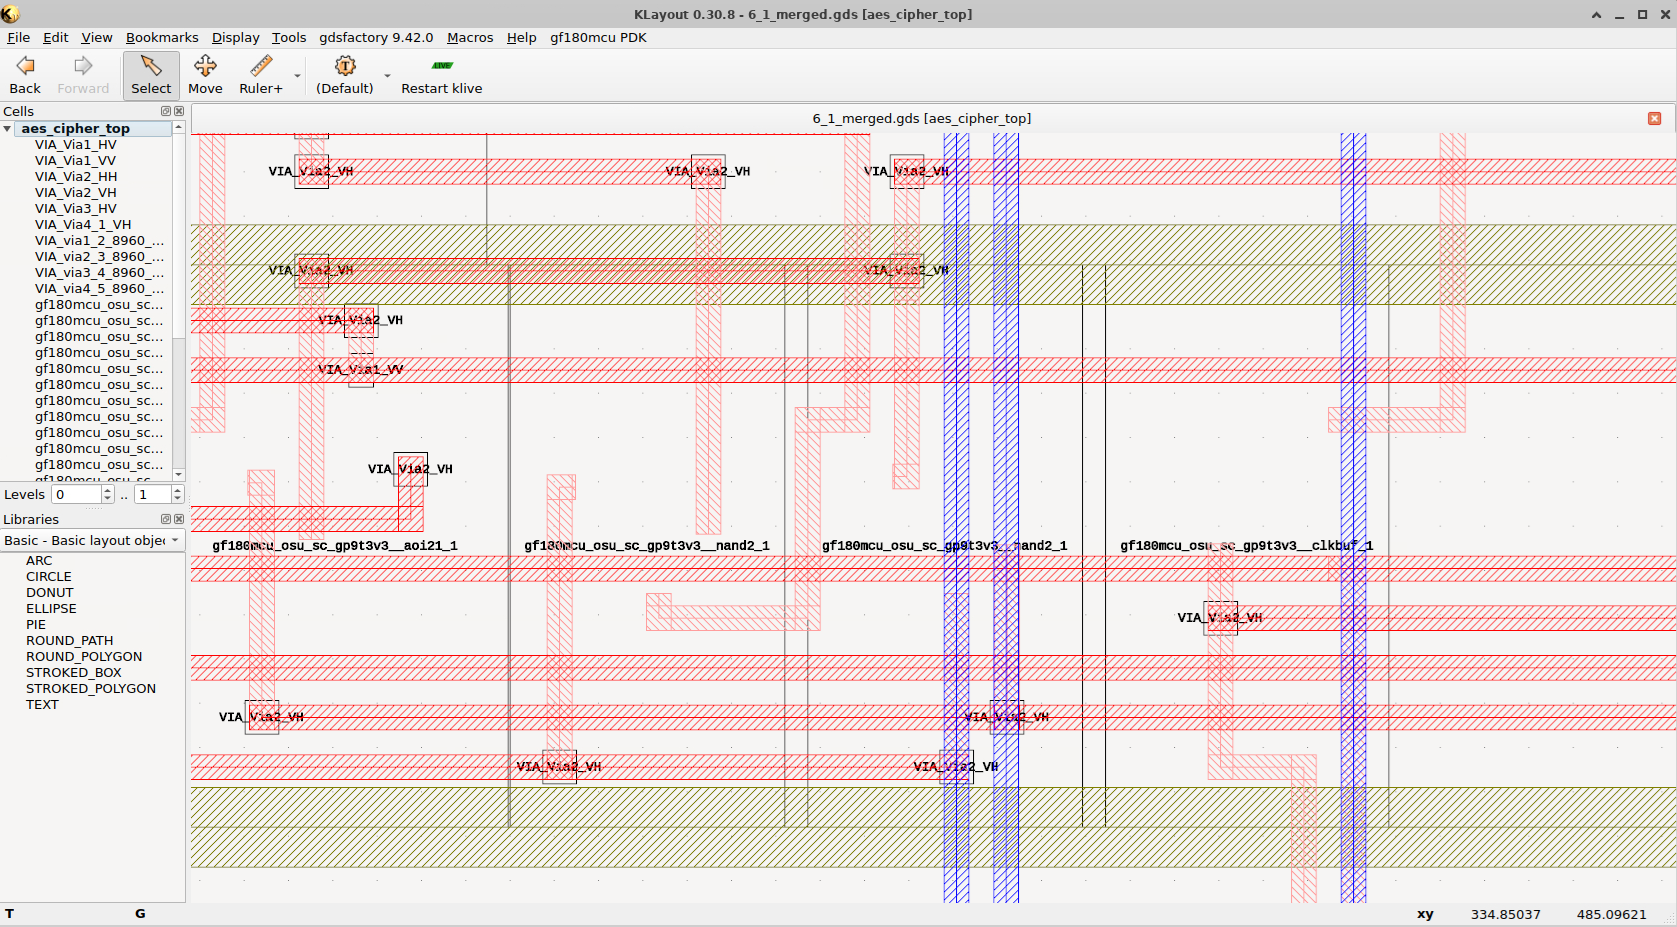
\includegraphics[width=0.90\textwidth]{klayout-osu.png}
    \caption{Zoomed-in view of the generated GDS layout in KLayout, showing the routing layers and visible OSU standard cells inside the final design.}
    \label{fig:klayout_osu_layout}
\end{figure}


% ============================================================
\section{Debugging and Problem Resolution}

This section documents several practical issues encountered during the setup and execution of the OpenROAD workflow, together with the corresponding debugging steps and solutions.
Because this workflow integrates multiple tools, scripts, libraries, and container configurations, various compatibility and runtime problems may appear during execution. Recording these issues and their corresponding solutions is important because it helps future users reproduce the workflow more reliably and understand the reasoning behind each modification.


\subsection{Incorrect \texttt{ABC\_DRIVER\_CELL} and \texttt{MIN\_BUF\_CELL} Names}

\textbf{Problem:}  
The original platform configuration used incorrect cell-name expressions for the buffer cells:

\begin{lstlisting}
export ABC_DRIVER_CELL = gf180mcu_osu_sc_gp9t3v3$(TRACK_OPTION)$(POWER_OPTION)__buf_4
export MIN_BUF_CELL_AND_PORTS = gf180mcu_osu_sc_gp9t3v3$(TRACK_OPTION)$(POWER_OPTION)__buf_1 A Y
\end{lstlisting}

\textbf{Debugging:}  
The correct buffer-cell names were checked from the Liberty files using:

\begin{lstlisting}
grep -i "cell.*buf_4" .../lib/*.lib | head -5
\end{lstlisting}

\textbf{Solution:}  
The cell names were corrected as follows:

\begin{lstlisting}
export ABC_DRIVER_CELL = gf180mcu_osu_sc_gp9t3v3__buf_4
export MIN_BUF_CELL_AND_PORTS = gf180mcu_osu_sc_gp9t3v3__buf_1 A Y
\end{lstlisting}

\subsection{Broken Final Line in the Platform \texttt{config.mk}}

\textbf{Problem:}  
The last line of the platform configuration file was corrupted:

\begin{lstlisting}
-include $(GF180_PRIVATE_DIR)/private.mk80_PRIVATE_DIR)/private.mk
\end{lstlisting}

\textbf{Solution:}  
The line was corrected to:

\begin{lstlisting}
-include $(GF180_PRIVATE_DIR)/private.mk
\end{lstlisting}



\subsection{Resolving the SITE Definition Mismatch for OSU Library Integration}

\textbf{Problem:}  
During detailed placement, the flow failed because the site definition used by the OSU standard-cell library was not consistent with the default GF180 technology LEF used in the platform setup. As a result, the placement rows generated from the platform technology definition did not match the physical site requirements of the OSU cells, which led to complete detailed-placement failure:

\begin{lstlisting}
Diamond Move Success: 0 (0.00%)
Total Placement Failures: 11004
[ERROR DPL-0036] Detailed placement failed
\end{lstlisting}

\textbf{Debugging:}  
To identify the cause of the failure, the site definitions in the OSU library LEF and the default GF180 technology LEF were compared:

\begin{lstlisting}
grep -A5 "^SITE" .../lef/gf180mcu_osu_sc_gp9t3v3_site.lef
grep -A5 "^SITE" .../lef/gf180mcu_5LM_1TM_9K_9t_tech.lef
\end{lstlisting}

The OSU library used the following site size:

\begin{lstlisting}
SIZE 0.56 BY 6.35
\end{lstlisting}

whereas the default GF180 platform technology LEF used:

\begin{lstlisting}
SIZE 0.56 BY 5.04
\end{lstlisting}

This mismatch indicated that the placement site used by the platform was incompatible with the OSU cell library in this integration setup.

\textbf{Solution:}  
Instead of modifying the original technology LEF directly, a separate adapted technology LEF file was created for the OSU-based flow. In this file, the site name and site size were updated so that the platform row definition matched the OSU library site definition:

\begin{lstlisting}
cp .../gf180mcu_5LM_1TM_9K_9t_tech.lef \
   .../gf180mcu_5LM_1TM_9K_9t_tech_osu.lef

sed -i 's/SITE GF018hv5v_green_sc9/SITE gf180mcu_osu_sc_gp9t3v3/g' \
    .../gf180mcu_5LM_1TM_9K_9t_tech_osu.lef

sed -i 's/SIZE 0.56 BY 5.04/SIZE 0.56 BY 6.35/g' \
    .../gf180mcu_5LM_1TM_9K_9t_tech_osu.lef

sed -i 's/END GF018hv5v_green_sc9/END gf180mcu_osu_sc_gp9t3v3/g' \
    .../gf180mcu_5LM_1TM_9K_9t_tech_osu.lef
\end{lstlisting}

The design configuration was then updated to use the adapted technology LEF:

\begin{lstlisting}
export TECH_LEF = .../gf180mcu_5LM_1TM_9K_9t_tech_osu.lef
\end{lstlisting}

\textbf{Remarks:}  
This modification is used here as an integration step to make the OpenROAD platform technology definition consistent with the OSU library site definition. It is not presented as a universal modification to the GF180 platform, but as a library-specific compatibility adjustment for this worked example.



% ============================================================

\end{document}
